% !Mode:: "TeX:DE:UTF-8:Main"

\documentclass{beamer}\usepackage[]{graphicx}\usepackage[]{color}
%% maxwidth is the original width if it is less than linewidth
%% otherwise use linewidth (to make sure the graphics do not exceed the margin)
\makeatletter
\def\maxwidth{ %
  \ifdim\Gin@nat@width>\linewidth
    \linewidth
  \else
    \Gin@nat@width
  \fi
}
\makeatother

\definecolor{fgcolor}{rgb}{0.345, 0.345, 0.345}
\newcommand{\hlnum}[1]{\textcolor[rgb]{0.686,0.059,0.569}{#1}}%
\newcommand{\hlstr}[1]{\textcolor[rgb]{0.192,0.494,0.8}{#1}}%
\newcommand{\hlcom}[1]{\textcolor[rgb]{0.678,0.584,0.686}{\textit{#1}}}%
\newcommand{\hlopt}[1]{\textcolor[rgb]{0,0,0}{#1}}%
\newcommand{\hlstd}[1]{\textcolor[rgb]{0.345,0.345,0.345}{#1}}%
\newcommand{\hlkwa}[1]{\textcolor[rgb]{0.161,0.373,0.58}{\textbf{#1}}}%
\newcommand{\hlkwb}[1]{\textcolor[rgb]{0.69,0.353,0.396}{#1}}%
\newcommand{\hlkwc}[1]{\textcolor[rgb]{0.333,0.667,0.333}{#1}}%
\newcommand{\hlkwd}[1]{\textcolor[rgb]{0.737,0.353,0.396}{\textbf{#1}}}%
\let\hlipl\hlkwb

\usepackage{framed}
\makeatletter
\newenvironment{kframe}{%
 \def\at@end@of@kframe{}%
 \ifinner\ifhmode%
  \def\at@end@of@kframe{\end{minipage}}%
  \begin{minipage}{\columnwidth}%
 \fi\fi%
 \def\FrameCommand##1{\hskip\@totalleftmargin \hskip-\fboxsep
 \colorbox{shadecolor}{##1}\hskip-\fboxsep
     % There is no \\@totalrightmargin, so:
     \hskip-\linewidth \hskip-\@totalleftmargin \hskip\columnwidth}%
 \MakeFramed {\advance\hsize-\width
   \@totalleftmargin\z@ \linewidth\hsize
   \@setminipage}}%
 {\par\unskip\endMakeFramed%
 \at@end@of@kframe}
\makeatother

\definecolor{shadecolor}{rgb}{.97, .97, .97}
\definecolor{messagecolor}{rgb}{0, 0, 0}
\definecolor{warningcolor}{rgb}{1, 0, 1}
\definecolor{errorcolor}{rgb}{1, 0, 0}
\newenvironment{knitrout}{}{} % an empty environment to be redefined in TeX

\usepackage{alltt}
\usepackage{tikz}
\usepackage[english]{babel}
\usepackage[utf8]{inputenc}
\usepackage[T1]{fontenc}
\usepackage{lipsum}

\usepackage{textpos} 
\usepackage{hyperref}
\usepackage{amsmath,amsthm,amsfonts,nicefrac,mathabx,amssymb}
\usepackage[subnum]{cases}
\usepackage{calligra, mathrsfs}
%\usepackage{natbib}
\usepackage{booktabs}
%\bibpunct{(}{)}{;}{a}{,}{,}

\usepackage{helvet}
\usepackage{graphicx}
\usepackage{color}
\usepackage{multirow,dcolumn}
\usepackage{ragged2e}
\usepackage{xcolor}
\usepackage{colortbl}
\usepackage{booktabs}
\usepackage{url}
\usepackage{bibentry}
\usepackage{chngcntr}

\usetheme{Gesis}


\newcommand{\eqname}[1]{\tag*{#1}} %equation title

%new math cal fonds
\newenvironment{frcseries}{\fontfamily{frc}\selectfont}{}
\newcommand{\textfrc}[1]{{\frcseries#1}}
\newcommand{\mathfrc}[1]{\text{\textfrc{#1}}}

\setcounter{tocdepth}{1}
\setbeamercolor*{section in toc}{fg=hellgrau}
\setbeamertemplate{bibliography item}[default]


\setcounter{secnumdepth}{3}
\setcounter{tocdepth}{3}


\newcommand{\E}[1]{\text{E}\left(#1\right)}
\newcommand{\V}[1]{\text{V}\left(#1\right)}
\newcommand{\Vest}[1]{\widehat{\text{V}}\left(#1\right)}
\newcommand{\MSE}[1]{\text{MSE}\left(#1\right)}
\newcommand{\COV}[2]{\text{COV}\left(#1,\,#2\right)}

\newcommand{\RN}[1]{%
  \textup{\uppercase\expandafter{\romannumeral#1}}%
}


\makeatletter

%%%%%%%%%%%%%%%%%%%%%%%%%%%%%% LyX specific LaTeX commands.
\providecommand{\LyX}{\texorpdfstring%
  {L\kern-.1667em\lower.25em\hbox{Y}\kern-.125emX\@}
  {LyX}}

%%%%%%%%%%%%%%%%%%%%%%%%%%%%% Textclass specific LaTeX commands.
% this default might be overridden by plain title style
 \newcommand\makebeamertitle{\frame{\maketitle}}%
 % (ERT) argument for the TOC
 \AtBeginDocument{%
   \let\origtableofcontents=\tableofcontents
   \def\tableofcontents{\@ifnextchar[{\origtableofcontents}{\gobbletableofcontents}}
   \def\gobbletableofcontents#1{\origtableofcontents}
 }




\title{Sample Theory}
\subtitle{Epidemiological Study Design and Statistical Methods}

\author{Stefan Zins - GESIS}
\date{12.12.2017}

% Gestaltungsvarianten
% Kopfbandfarbe "shaded" von weiß zu blau: 
% \setbeamertemplate{gesisheadband}[shaded]
% andere Farbwerte
% \gesisCIbluecolors % = Blau und Orange aus CI, Blau als heller Hintergrund
% \gesisCIcolors     % = Blau und Orange aus CI, Sand als heller Hintergrund
\IfFileExists{upquote.sty}{\usepackage{upquote}}{}
\begin{document}

\gesismaketitle % erzeugt Titelseite

\begin{frame}%[t]
  \frametitle{Content}
  
  \begin{itemize}
  \item Introduction
  %\item Populations
  \item Sampling Designs
  \item Planing
  \end{itemize}


\end{frame}

\section{Desgin Based Inferenz}



\begin{frame}{Population, Sample, and Sampling Design}

 \begin{itemize}
 \item[] 
 \begin{align}
 \mathcal{Y} = & \{ y_1{,}y_2{,}\,\ldots{,}\,y_k{,}\,\ldots{,}\,y_N \} \eqname{finite population of size $N$} \\
 \mathcal{U} = &\, \{ 1{,}2{,}\,\ldots{,}\,k{,}\,\ldots{,}\,N \} \eqname{sampling frame} \\
 \mathfrc{s} \subset &\, \mathcal{U} \eqname{sample of size $n$} \\
 \mathcal{P}(\mathcal{U}) & \eqname{all possible subsets of $\mathcal{U}$}
 \end{align}
 \item[]
\item[]
The discrete probability distribution $p(.)$ over $\mathcal{P}(\mathcal{U})$ is called
a \emph{sampling design} and  $\mathcal{G}=\{ \mathfrc{s} | \mathfrc{s} \in
\mathcal{P}(\mathcal{U}),\, p(\mathfrc{s}) > 0 \}$ is called the support of $p(.)$ with
$$
\sum_{\mathfrc{s} \in \mathcal{G}} p(\mathfrc{s}) = 1
$$
Hence, $p: \; \mathcal{G} \mapsto (0, 1]$.
 \end{itemize}
\end{frame}


\begin{frame}{Estimation}
\begin{align}
 \theta       & = f(\mathcal{Y})  \eqname{statistic of interest} \\
 \hat{\theta} & = f(\mathcal{Y}, \mathfrc{s} )  \eqname{estimator for $\theta$} \\
 \E{\hat{\theta}} & = \sum_{\mathfrc{s} \in \mathcal{G}} p(\mathfrc{s}) f(\mathcal{Y}, \mathfrc{s} )   \eqname{expected value of $\hat{\theta}$} \\
 \V{\hat{\theta}}   & =  \E{\hat{\theta}^2} -  {\E{\hat{\theta}}}^2 \eqname{variance of  $\hat{\theta}$} 
\end{align}
 $\E{.}$, $\V{.}$, and $\MSE{.}$ are always with respect to the sampling design $p()$ and
 an estimator is said to be unbiased if
 $$ \E{\hat{\theta}} = \theta\;. $$
\end{frame}


\begin{frame}{Representative Sample}
\onslide*<1-2>{What is a representative sample? \newline}
\onslide*<2>{The popular concept of a representative sample it that the sample is a \emph{miniature} of the population.}

\onslide<3-4>{However, what do we really want?}
\onslide<4>{\newline We want to estimate a statistic of interest with a certain level of precision 
 and if the level of precision is high enough we say our estimation \emph{strategy} is representative.}


\end{frame}

\begin{frame}{Examples}
Does this

Difference of mean
Regression

\end{frame}

\begin{frame}{Inclusion Probabilities}

$V(\theta)=f(y,\Sigma)$

not only the weights 

Estimation with weights
Inference requires Variance estimaion

Design Weight 

\end{frame}


\section{Sampling Designs}

\begin{frame}{Sampling Frames}
Access to target population

Address    Samples (Register that list all sampling units)
Telelephon Samples (Not fully known but all possible entries)



\end{frame}


\begin{frame}{Sampling Methods}
Probability based Samples

Known and Accesable Sampling Frame
Desgin should be measureable
$\pi_{k}>0  \forall k \in \mathcal{U}$
$\pi_{kl}>0 \forall k \neq l \in \mathcal{U}$



Nonprobability based Samples

Examples
Convenience Samples
Purposive   Samples
Opt-in      Samples (Online) Access Panels - Addertising on webpages
Quota       Samples

The selection process is often to complex to model it
Assumptions are made over the data itself (model-based inference)

\end{frame}



%alter

\begin{frame}{Techniques for probabilitic Sampling}
A set of rules (algrithm)

\emph{Simple} Random Sampling
All samples not sample elements have the same probability of being selected.
p(s) is a constant for all s

Unequal Probability Sampling



Systematic Sampling

Random Routes

Cite Tille

\end{frame}


\begin{frame}{Stratification}
A Population of 100 elements is stratified into $H=6$ strata.

%fig.keep='all',fig.show='asis'
\onslide*<1>{
\begin{knitrout}
\definecolor{shadecolor}{rgb}{0.969, 0.969, 0.969}\color{fgcolor}
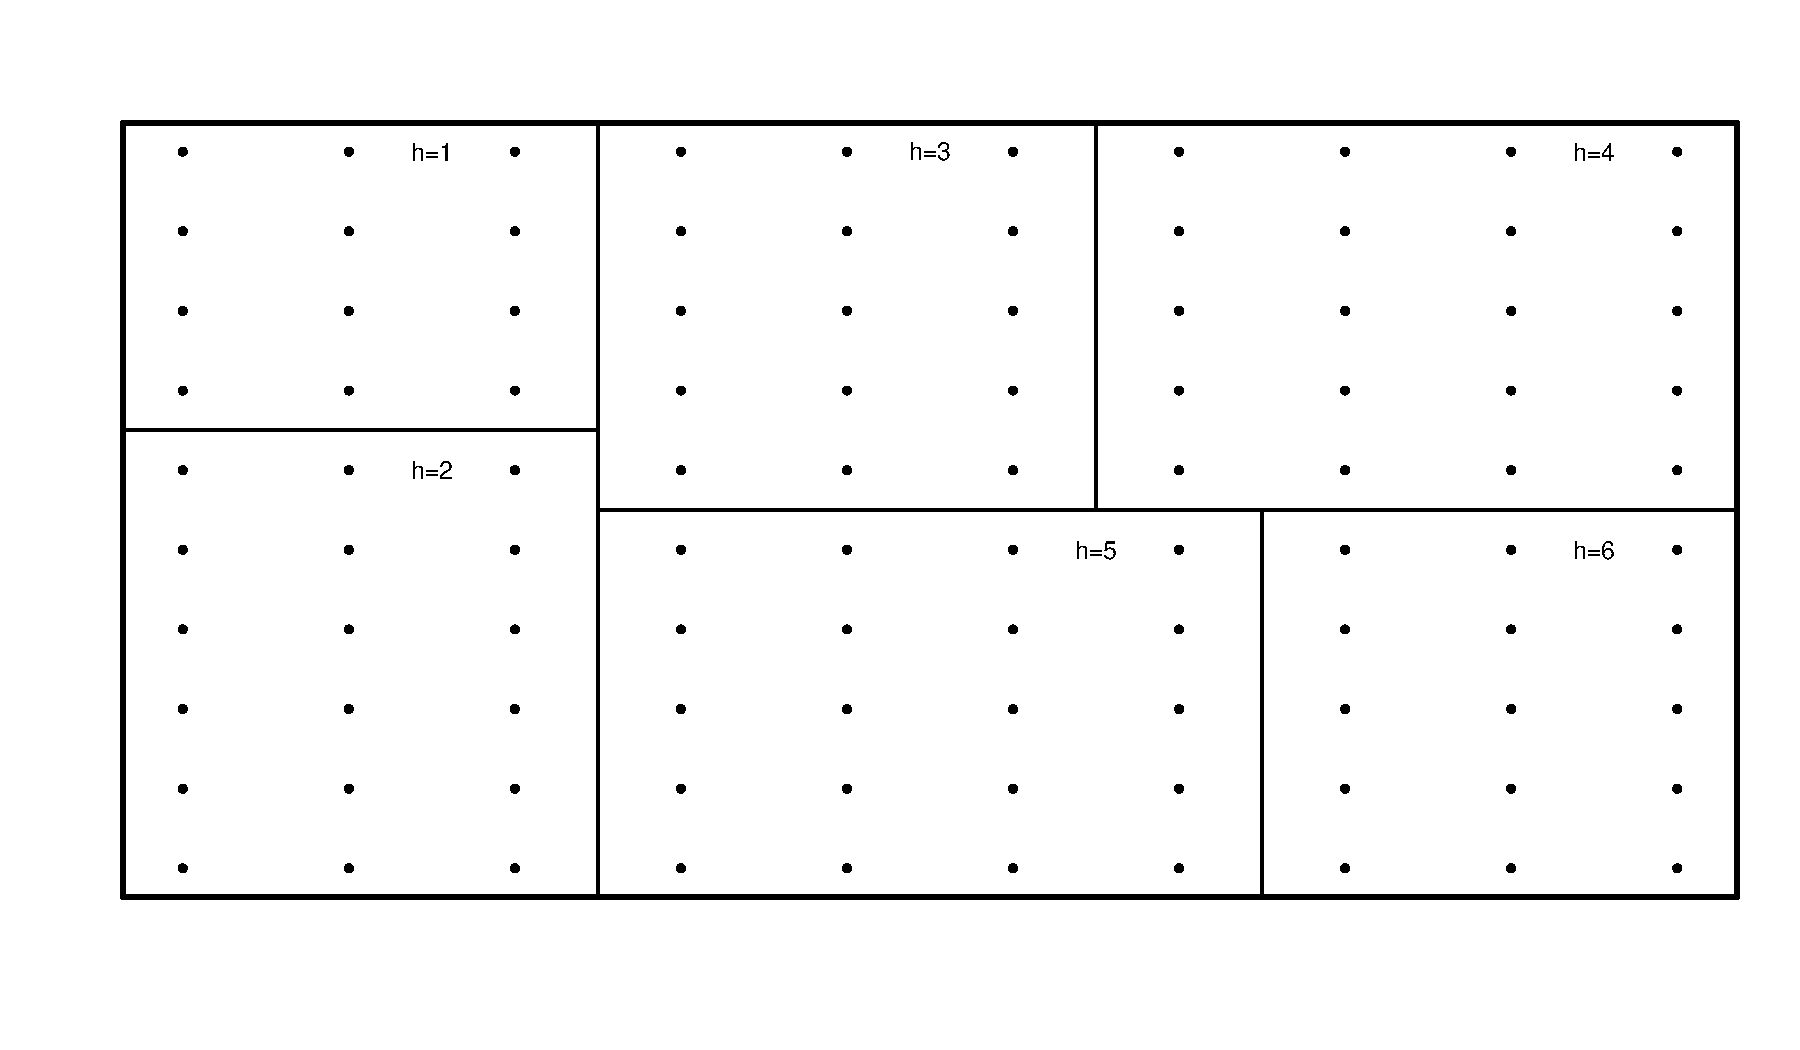
\includegraphics[width=.85\linewidth]{figure/StratPlot1-1} 

\end{knitrout}
}
\onslide<2>{
14 elements are selected population and their allocation is given by
\begin{tabular}{cccccc}
$n_1$ = 2  & $n_2$ = 3  & $n_3$ = 2  & $n_4$ = 3 & 
 $n_5$ = 3&  $n_6$ = 2\\
\end{tabular}

\begin{knitrout}
\definecolor{shadecolor}{rgb}{0.969, 0.969, 0.969}\color{fgcolor}
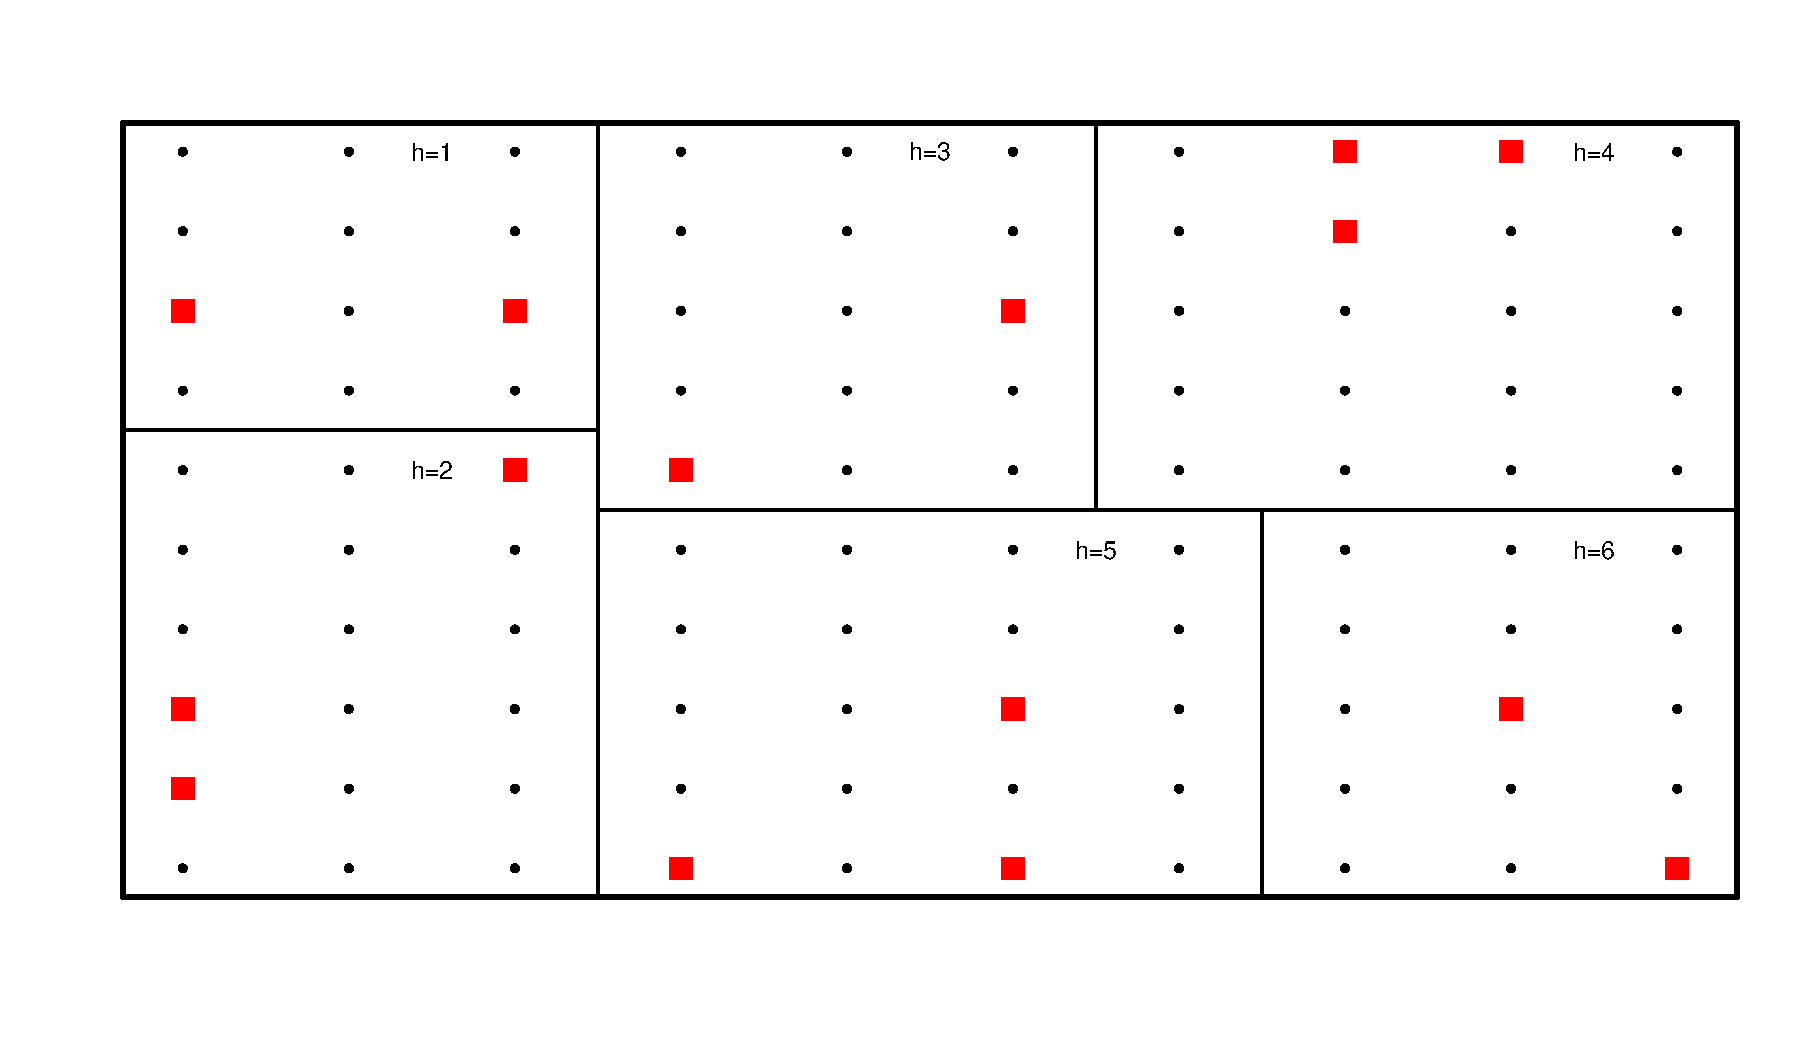
\includegraphics[width=.85\linewidth]{figure/StratPlot2-1} 

\end{knitrout}
}
\end{frame}


% \begin{frame}{Issues with Stratification}
% \begin{itemize}
% \item<1-> Why should stratification be used?
% \begin{itemize}
% \item<2-> To reduce the sampling variance of estimators.
% \item<2-> Sometimes it is necessary because of organizational reasons, (e.g. no joint sampling frame).
% \end{itemize}
% \item<3-> How should the population be stratified?
% \begin{itemize}
% \item<4-> A \emph{good} set of variables needs to be found for stratification.
% \item<4-> The number of strata has to be decided.
% \end{itemize}
% \item<5-> How should the overall sample size be allocated to the strata?
% \begin{itemize}
% \item<6-> Achieve proportionality between sample and population (i.e. the frame)
% \item<6-> Fulfill precision constraints for certain estimation domains
% \end{itemize}
% \end{itemize}
% 
% \end{frame}

\begin{frame}{Defining the Strata}

Sratification can redure the sampling variance of estimators.

  % \begin{table}\caption{Population ANOVA}
  % \begin{tabular}{l | l | l }
  % Source & df & Sum of Squares  \\
  % \hline 
  %  Between strata         & $H-1$ & $\text{SSB}  = \sum_{h=1}^H N_h ( \mu_{h} - \mu  )^2$  \\ 
  %  Within  strata         & $N-H$ & $\text{SSW}  = \sum_{h=1}^H (N_h-1) V_{h}^2$  \\
  %  Total,  about  $\mu_y$ & $N-1$ & $\text{SSTO} = (N-1) V^2$ \\
  % \end{tabular}
  % \end{table}

The more homogeneous the strata are the higher is the gain in efficiency from using stratified simple random sample sampling (StrSRS) instead of SRS. Because then SSW (variance within) is
considerably small in contrast to SSB (variance between). This is called
the  effect of stratification. 

Optimal Stratfication

\end{frame}
% %survey imperfections 
%$N_h > 2$ variance estimation is difficult 
% $\V{\hat{\theta}}$

\begin{frame}{Allocation Methods}
For all $h = 1{,}\,\ldots{,}\,H$
 \begin{equation*} \arraycolsep=1.4pt\def\arraystretch{2.2}
  n_h = \left\{ \begin{array}{l r}
        \dfrac{n}{H}  &\; \text{equal allocation} \\
        \dfrac{N_h}{N}  n    &\; \text{proportional allocation} \\
        \dfrac{N_h V_{h}}{\sum_{h=1}^H N_h V_{h} }  n  &\; \text{optimal allocation} 
  \end{array}\;\right.{,}
 \end{equation*}
 where $\overline{c}_h$ are average cost of selecting a element from stratum $h$ and $c=\sum_{h=1}^H n_h \overline{c}_h$ are the total costs of the survey. For the cost-optimal allocation $c$ is given, not $n$.
% 
% Variants of proportional allocation to totals
% proportional to y or auxiliar variable
% %the rounding probelem
\end{frame}


\begin{frame}{Clustering}

A Population of 100 elements is clustered into $N_{\RN{1}}=6$ cluster
%fig.keep='all',fig.show='asis'
\onslide*<1>{
\begin{knitrout}
\definecolor{shadecolor}{rgb}{0.969, 0.969, 0.969}\color{fgcolor}
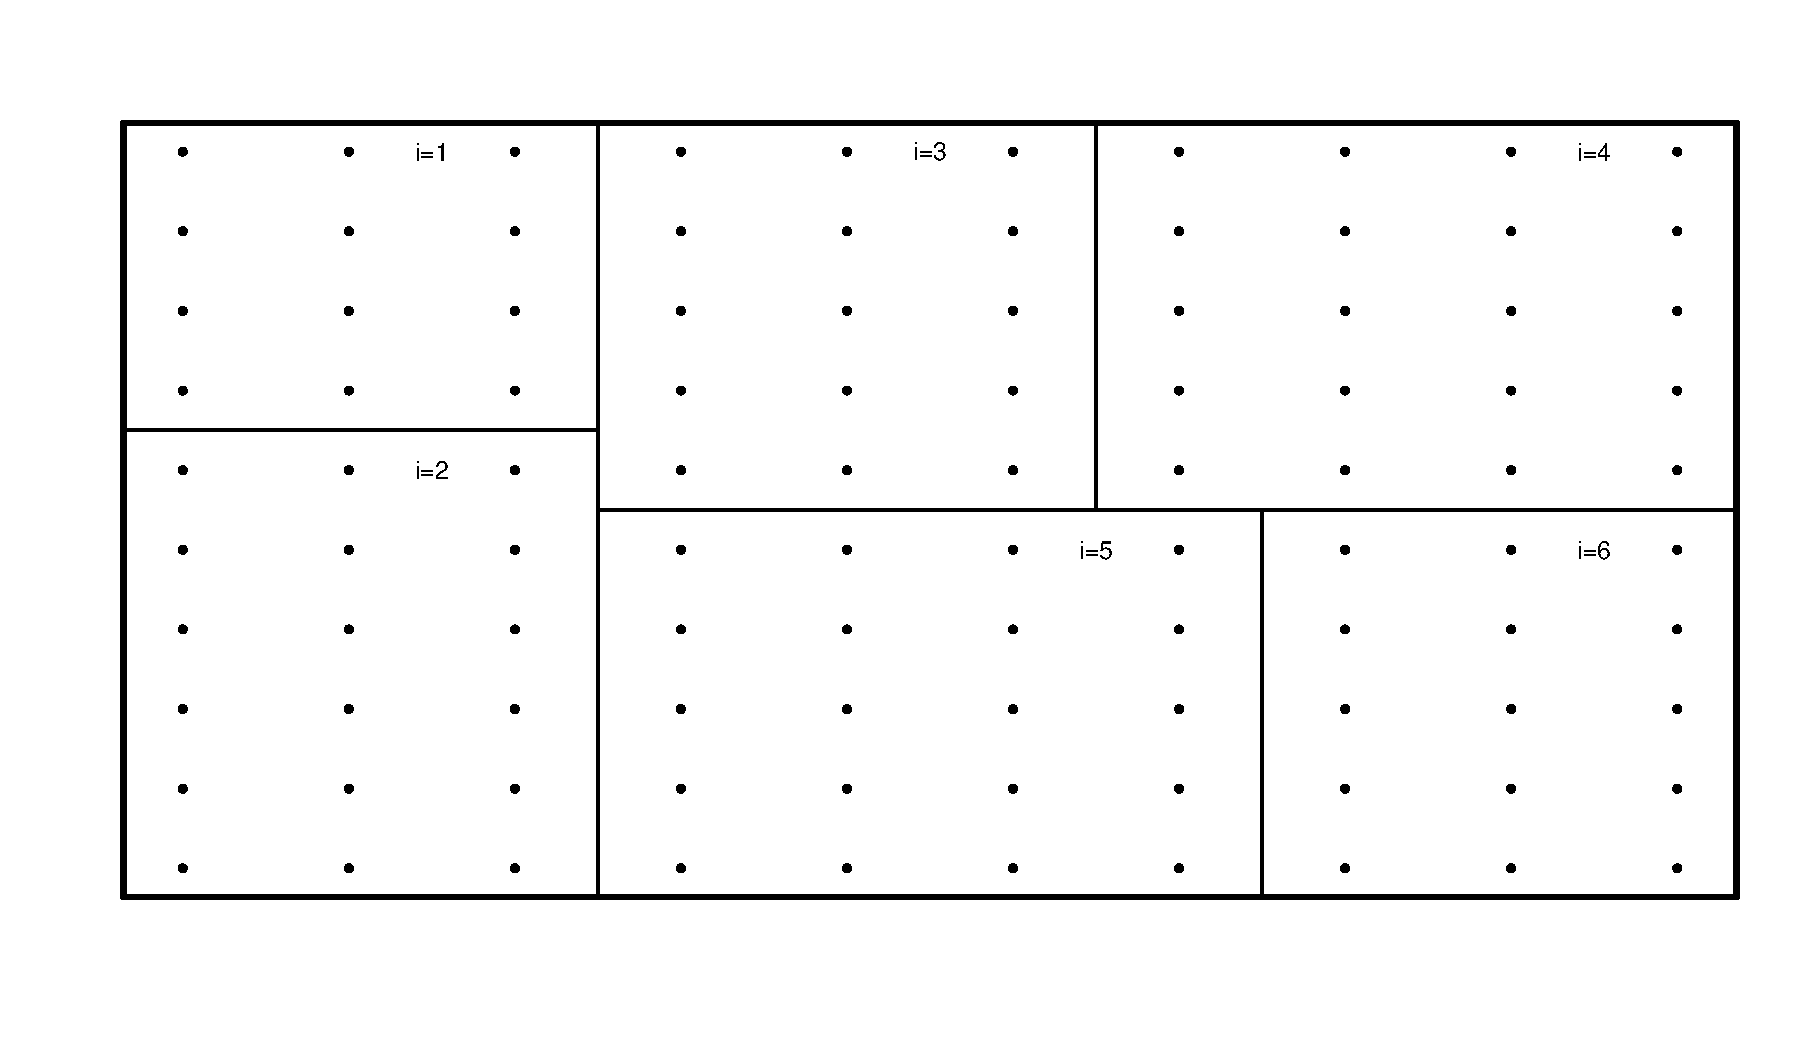
\includegraphics[width=.85\linewidth]{figure/CluPlot1-1} 

\end{knitrout}
}\onslide<2>{
and $n_{\RN{1}}=2$ clusters are selected from the population.
\begin{knitrout}
\definecolor{shadecolor}{rgb}{0.969, 0.969, 0.969}\color{fgcolor}
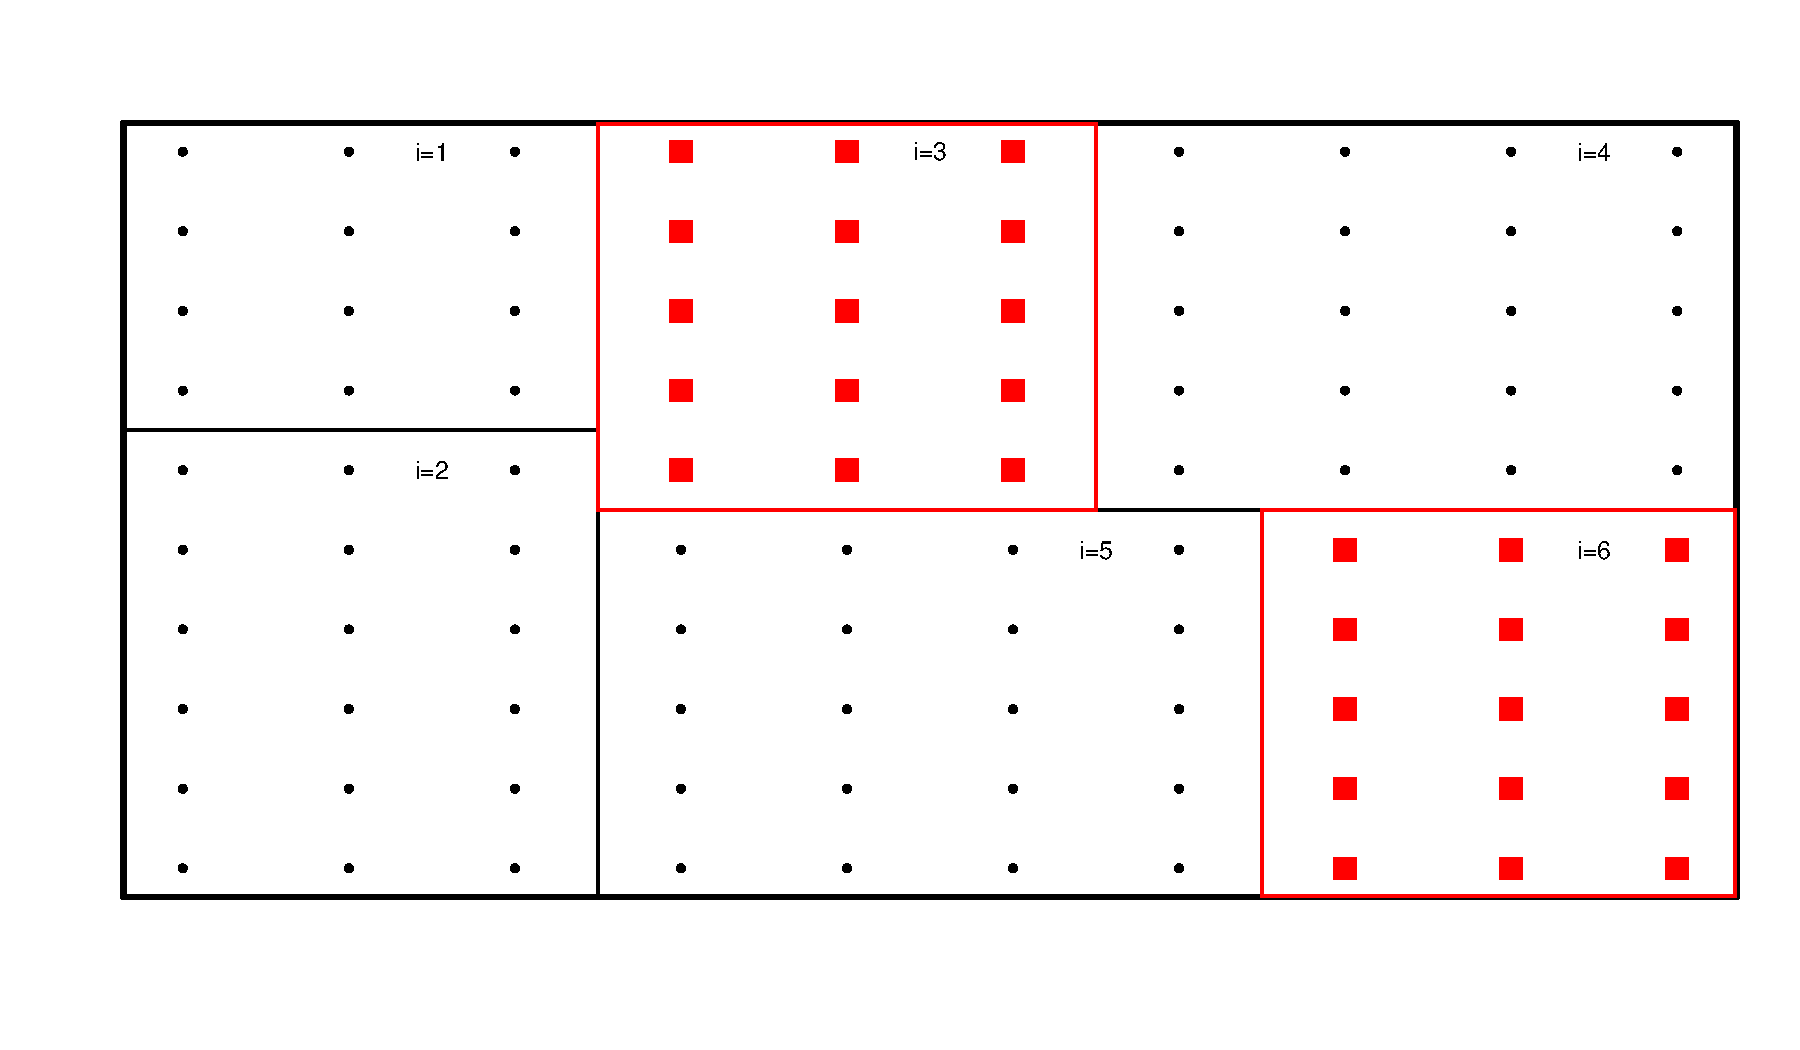
\includegraphics[width=.85\linewidth]{figure/CluPlot2-1} 

\end{knitrout}
}
\end{frame}


\begin{frame}{Cluster Sampling}
\begin{itemize}
\item[]<1-> Sampling elementary units is often not feasible (e.g. persons or businesses). Maybe there is no uniform sampling frame available to select them from, or it would be costly to do, because the selected elements would scatter to much over the a certain area and travel costs of interviewers would be to high. 

\item[]<2-> Thus, it is very common to select clusters, so called \emph{primary sampling units} (PSU's) that are populated by \emph{secondary sampling units} (SSU's).

\item[]<3-> Cluster sampling makes it still possible to obtain unbiased estimates but it can have a big influence on the variance. 
\end{itemize}

\end{frame}



\begin{frame}{Example}
Compare Variances

Cluster sampling  by dnum
Stratified Sampling  dnum
%summary statistcs on apipop
\end{frame}



%\section{Complex Sampling Designs - Two Stage Sampling}

\begin{frame}{Two Stage Sampling}
% A Population of 100 elements is clustered into $N_{\RN{1}}=6$ clusters
% and $n_{\RN{1}}=n_I$ clusters (PSU) are selected at the first sampling stage
%\onslide*<1>{
\begin{knitrout}
\definecolor{shadecolor}{rgb}{0.969, 0.969, 0.969}\color{fgcolor}
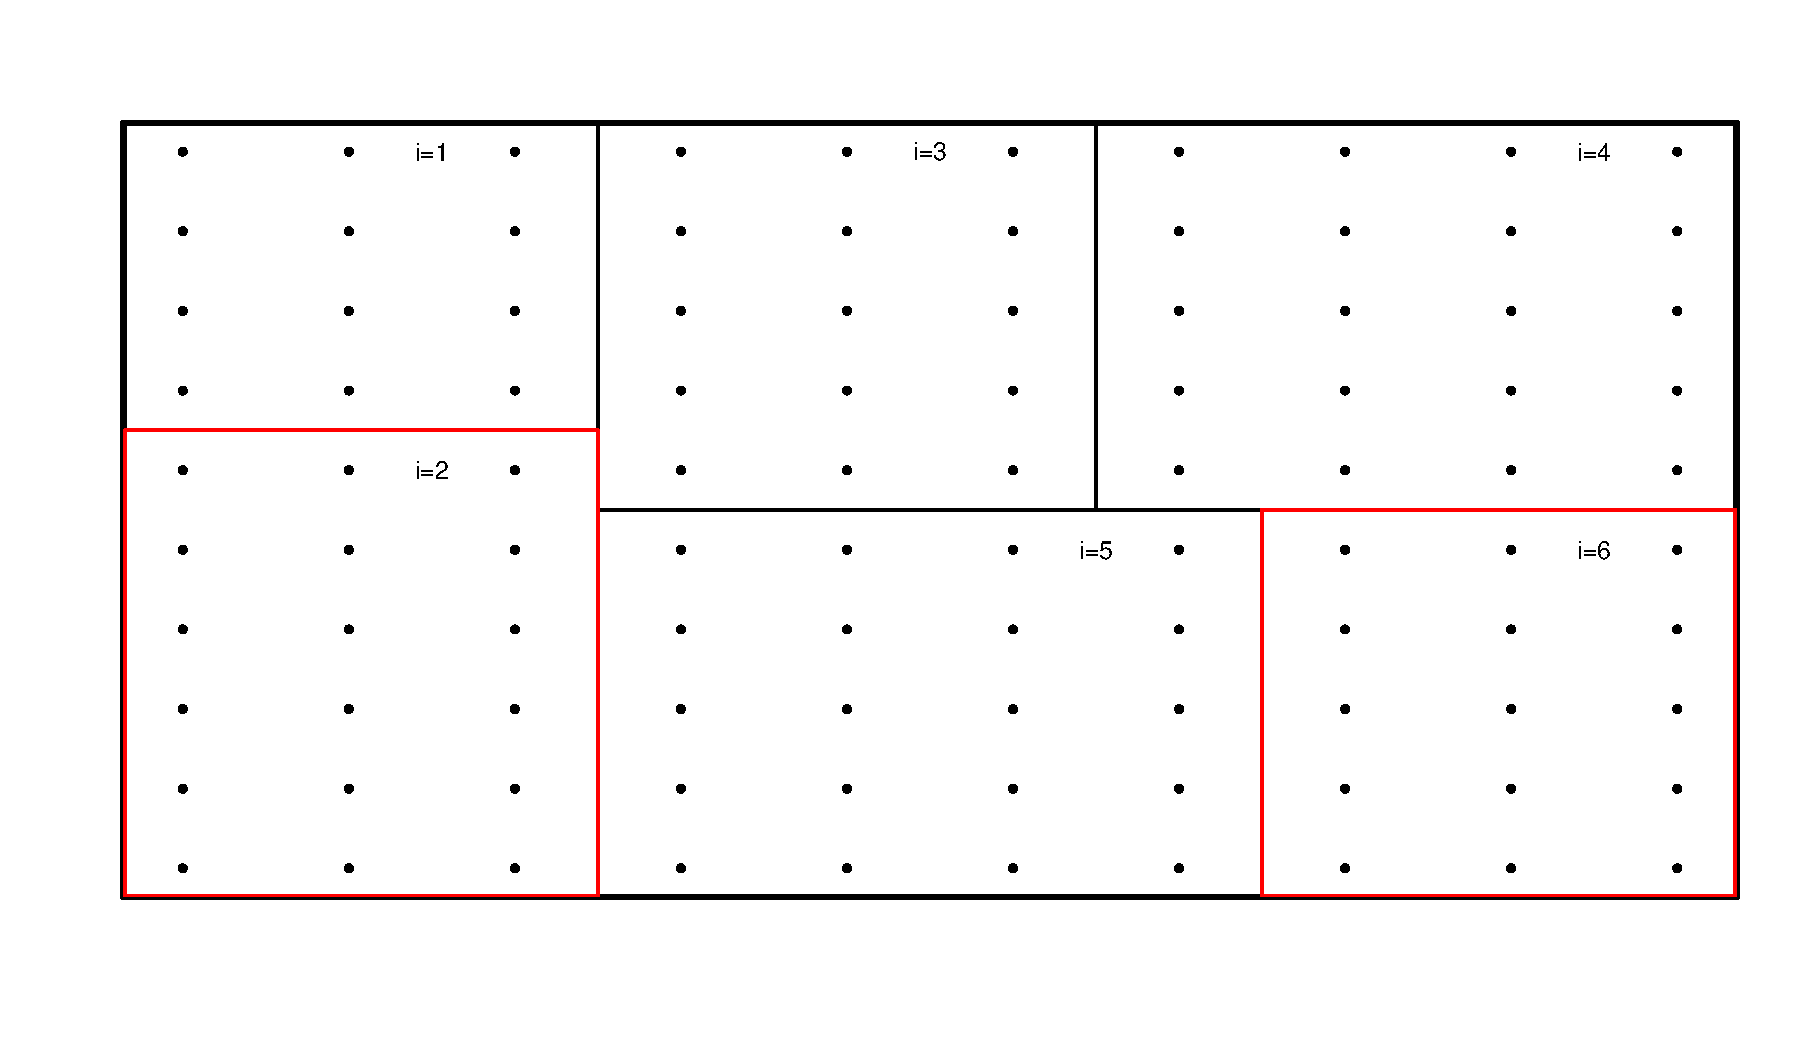
\includegraphics[width=.85\linewidth]{figure/CluPlot1_2-1} 

\end{knitrout}

% }\onslide<2>{
% and $n_{i}=4$ elements are selected from each sampled cluster.
% <<CluPlot2.2,echo=FALSE,fig.width=12,out.width='.85\\linewidth'>>=
% <<CluPlot1.2>>
% for(i in sam.str) {
%       s_i <- sample(length(strata.Xs[[i]]), n_i)
%       points(x=strata.Xs[[i]][s_i],y=strata.Ys[[i]][s_i],pch=15,col=2,cex=2)
% }
% @
% }
% 
% 



\end{frame}


\begin{frame}{Two Stage Sampling}
 \begin{description}
 \item[First  stage] A sample $\mathfrc{s}_{\RN{1}}$ of PSU's is drawn from $\mathcal{U}_{\RN{1}}$ according to some sampling design $p_{\RN{1}}(.)$
 \item[Second stage] For every $i \in \mathfrc{s}_{\RN{1}}$ a sample $\mathfrc{s}_i$ of SSU's is selected from $\mathcal{U}_i$ according to some design $p_i(.|\mathfrc{s}_{\RN{1}})$
 \end{description}
 The resulting sample of SSU's is denote $\mathfrc{s}= \bigcup_{i \in \mathfrc{s}_{\RN{1}}} \mathfrc{s}_i $.
 In general, samples $\mathfrc{s}_i$ are selected independently of each other, thus, the inclusion probability of a element $k \in \mathcal{U}_i$ is
$$\pi_k=\pi_{\RN{1}i}\pi_{k|i}\;,$$
where $\pi_{\RN{1}i}$ is the probability of selecting the $i$-th PSU and $\pi_{k|i}$  the probability of selecting
the $k$-th SSU in the $i$-th PSU.
\end{frame}


\begin{frame}{Sample Size Determination}
Samples Size are planned with a specific estimator in mind

Complex Problem for Multivariate Surveys

the minimum sample size under a certain precision requirements

The variance or MSE of an estimator


\end{frame}

\begin{frame}

\begin{beamercolorbox}[wd=\paperwidth,center,sep=1cm]{gesisdarkbgbox}
   Vielen Dank für die Aufmerksamkeit
\end{beamercolorbox}
\end{frame}

\end{document} 
